\documentclass{article}

\usepackage[top=1in, bottom=1.25in, left=1.25in, right=1.25in]{geometry}
\usepackage{algpseudocode}
\usepackage{algorithm}
\usepackage{graphicx}
\usepackage{amsmath}
\usepackage{amssymb}
\usepackage{url}
\usepackage{booktabs}
\usepackage{pgfplots}
\pgfplotsset{compat=1.14}

\begin{document}

\title{Big Brother: Multi-camera Object Tracking}

\author{
  Mohit Deshpande\\
  The Ohio State University\\
  \texttt{deshpande.75@osu.edu}
  \and
  Brad Pershon\\
  The Ohio State University\\
  \texttt{pershon.1@osu.edu}
}

\date{}

\maketitle


\section{Introduction}
Cameras are ever present in our society. They are on traffic lights, on top of buildings, inside buildings, and on vehicles. Millions of dollars go to law enforcement and cities to help stop crime using new surveillance systems~\cite{surveillance}. Even universities are including cameras in their bus systems~\cite{cabs}. With this massive coverage of cameras, many of them overlap with each other, e.g., the field-of-view of a camera on a building might overlap with that of the camera on an adjacent building. In the event of a crime, law enforcement check all of these cameras and must manually track the perpetrator through potentially hundreds of cameras~\cite{surveillance}. Instead, we present an automated solution, called \texttt{BigBrother}, that can follow a target across any number of cameras. 

\section{BigBrother}
\label{sec:bigbrother}
The problem of object tracking through multiple cameras $\{\mathcal{C}_1,\dots,\mathcal{C}_N\}$, given a target $T$ in one camera, is to find and track that target in the other cameras. For simplicity, we assume that the target $T$ is first identified in $\mathcal{C}_1$ and call this the \textbf{primary camera}. We immediately start mean-shift tracking for the centroid of the target's bounding box. This mean shift produces new coordinates for the target, and we can transform these coordinates to other cameras using a homography. We use a novel multi-scale variant of covariance tracking to match the target in the non-primary camera, where the initial covariance matrix is taken from the feature matrix of the target. Algorithm~\ref{algo:bigbrother} describes our algorithm at a high level. The details are described in subsequent sections.

\begin{algorithm}
\caption{\texttt{BigBrother} Algorithm}\label{algo:bigbrother}
\begin{algorithmic}[1]
\Procedure{BigBrother}{$\mathcal{C}_1,\dots,\mathcal{C}_N,T$}
\State $\Sigma\gets \mathtt{feature\_cov}(\mathcal{C}_1, T)$\Comment{Covariance matrix for other cameras}
\State $B_i\gets\emptyset~~~~\forall i\in\{2,\dots,N\}$\Comment{Position of the target in other cameras}
\While{true}
    \State $T\gets \mathtt{meanshift}(\mathcal{C}_1, T)$\Comment{Update the target's position}

    \For{$i\gets 2$ to $N$}
        \State $T'\gets \mathcal{H}(\mathcal{C}_1, \mathcal{C}_i)\cdot T$\Comment{Transform coordinates using homography}
        \If{$T'\not\in\mathcal{C}_i$}
            \State $B_i\gets\emptyset$
            \State \textbf{continue}
        \EndIf
        \State $S\gets\mathtt{search\_region}(T')$\Comment{Define search region around mean-shift estimate}
        \State $B_i\gets\mathtt{multiscale\_cov\_track}(\Sigma, S)$\Comment{Find target in other cameras}
    \EndFor
\EndWhile
\EndProcedure
\end{algorithmic}
\end{algorithm}

\subsection{Homography}
\label{sec:homography}
To track a target across multiple cameras, we must have either complete 3D knowledge of the space of the cameras and their positioning in that space or, more simply, a homography between the cameras. The homography is simpler but can only be computed if the field-of-view of the cameras overlap. This is a critical assumption we make. Given the large number of cameras with overlapping field-of-views, this assumption is reasonable.

We compute a homography offline by selecting corresponding pixels between the two camera views, and a corner or feature detector may make pixel selection easier. We require at least 4 corresponding coordinates to compute the homography, however, for a better homography we used $32$ corresponding points. Each point is converted into homogeneous coordinates, and we solve the system of linear equations to produce the homography matrix $H$ between two camera views. This is shown as $\mathcal{H}(\mathcal{C}_1, \mathcal{C}_i)$ in Algorithm~\ref{algo:bigbrother}.

For robustness, we use a normalized direct linear transform: we normalize our points to have zero mean and shift the average distance of the resulting points to the origin is $\sqrt{2}$.

\subsection{Mean-Shift Tracking}
\label{sec:meanshift}
After computing the homography and identifying the region of interest in one camera frame, we can start mean-shift tracking~\cite{comaniciu2003kernel}. We assume the target's size is constant through the frames since we only track the centroid of the target. We use $16$ color bins for the color quantization, circular neighbors with a radius of $r=5$, and $h=25$ for the Epanechnikov profile. The reason we use a smaller radius is because our dataset has a smaller resolution.

At each frame of the mean-shift tracking, we use the homography to transform the mean-shift-tracked centroid into the other cameras. If the homography is accurate, we can determine if the target is in a particular camera frame. If the transformed points are outside of bounds of a camera frame, we ignore that camera and know that target is not present. However, if the points lie inside of a camera frame, we know the target is present in that particular camera frame.

\subsection{Covariance Tracking}
\label{sec:covariance}
To find the target in the other cameras, we use a novel multi-scale covariance tracking~\cite{porikli2006covariance}. One primary issue with covariance tracking is speed: we have to search the entire image. However, we can the transformed mean-shift estimate to narrow our search space. We take the bounding box points from the target in the primary camera frame and transform them into other camera frames. Since the homography might produces points that are skew, we take the axis-aligned rectangle to be our search area. This approach drastically limits our search. On average, we found a $94.3\%$ reduction in the number of pixels we must search.

The covariance matrix initialized from the original target in the primary camera. For our feature vector, we use the radial vector described in~\cite{porikli2006covariance} for each pixel in the search space.

\[
\mathbf{f} = \left[ ||(x', y')||~~I(x,y,1)~~I(x,y,2)~~I(x,y,3)\right]
\]

where $||(x', y')||$ is the radial distance from the center of the patch to the $j$th pixel in the patch. The last $3$ components are the RGB components of the pixel.

The covariance matrix is initialized with a fixed patch in the primary camera. However, in other cameras, the target may have different scales. The scale of the target will most likely be different in another camera, but there's a relation between the scale of the target in another camera and the primary camera. We propose a new multi-scale approach, inspired by the Region Proposal Network~\cite{ren2015faster}, that changes the scale of the sliding window in the search space. We define $K$ factors that scale the dimensions of the sliding window, equally along both dimensions. In addition to scaling the initial window, we also flip the dimensions, e.g., we use a sliding window of size $5\times 3$ as well as $3\times 5$, for every $K$ scaling factor. 

We perform covariance tracking by searching for the best, i.e., minimum-distance, match, computed using the metric described in~\cite{forstner2003metric}. However, doing this for $K$ filters and flipped dimensions, we will have $2\cdot K$ bounding boxes in the search space. We simply use non-maximal suppression, with an overlap ratio threshold of $0.05$, to reduce this number and select the bounding box of the smallest distance. The speed of this algorithm depends on the size of the search space $|S|$ and the number of scaling factors $K$. However, in practice, $K$ is much smaller compared to $|S|$, which dominates the time complexity.

We do not start mean-shift tracking in the other camera frame since we want to maintain the relationship of the target between several cameras. If we were to mean-shift track in all cameras, these would operate independently. This makes it impossible to pick up a target in a new camera since mean-shift would stop tracking after the target leaves a frame. To remedy this, we use the homography to connect the primary camera to the other cameras. If the target moves into the field-of-view of another camera, we will notice the project points will lie in the camera's field-of-view. This allows us to drop the target from a camera if it falls out of view and pick up the target in a camera if it comes into view.

\subsection{Work Allocation}
Mr. Pershon computed the homography $H$ between the two cameras. This was computed by manually matching correspondence points and solving the linear system of equations as described in Section~\ref{sec:homography}. He also implemented a highly-vectorized variant of mean-shift tracking for the primary camera.

Mr. Deshpande implemented the multi-scale covariance tracking and cross-camera interaction described in Section~\ref{sec:covariance}.

\subsection{Challenges}
\vspace{5pt}
\noindent\textbf{Co-planar points.} Homographies or other measurements are not entirely accurate; there is always some error associated with them. When transforming points between cameras, the transformed points are not that accurate. However, we can ameliorate this inconsistency by using more points when computing our homography. Since we use homographies for translating between different cameras, we only get reasonable results when the target is co-planar with the ground-plane. This is a limitation since many cameras, particularly indoor ones, do not have a high enough vantage point to satisfy the co-planar points requirements, or even approximate it reasonably.

\vspace{5pt}
\noindent\textbf{Loss of target in primary camera.} One assumption our algorithm makes is that the target remains in the same camera the entire during of our approach. If we lose the target in one camera but it is still present in another camera, we can simply switch from covariance tracking to mean-shift; that camera becomes our primary camera.

\vspace{5pt}
\noindent\textbf{Vastly varying target sizes.} The covariance matrix is computed from a patch of fixed size. When we perform the search, we compute the covariance of several scales. However, if our target does not match one of these scales, then we may miss the detection. However, since they're computed as a function of the original target's dimensions, we are likely to detect the target in the other cameras.

\section{Results}
\label{sec:results}
For our experiments, we used a video sample from the PETS 2001 dataset. The video has two surveillance cameras in the daytime, each with $384\times 144$ resolution. In particular, we track a moving van between these two cameras. A frame from both cameras at the same time step is shown in Figure~\ref{fig:dataset}. Figure~\ref{fig:results} shows an example frame from our algorithm. All experiments, accuracy and performance, were conducted on an Intel i7@3.2GHz processor with 16GB of RAM and no parallelization. Our algorithm was implemented in MATLAB.

\begin{figure}[t]
\centering
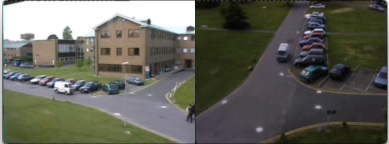
\includegraphics[width=\textwidth]{dataset.png}
\caption{Example frames from our dataset. Our experiments track the moving white van.}\label{fig:dataset}
\end{figure}

\begin{figure}[t]
\centering
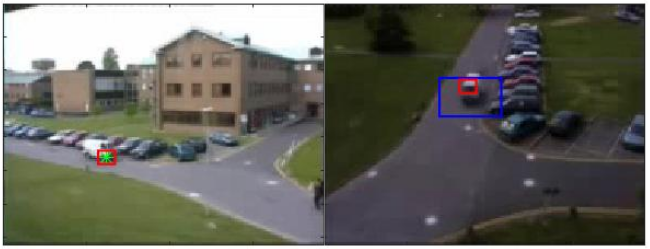
\includegraphics[width=\textwidth]{results.png}
\caption{Example frames from our algorithm. The blue box represents the projected search area, and the red box is the location of the target.}\label{fig:results}
\end{figure}

\begin{figure}[t]
\centering
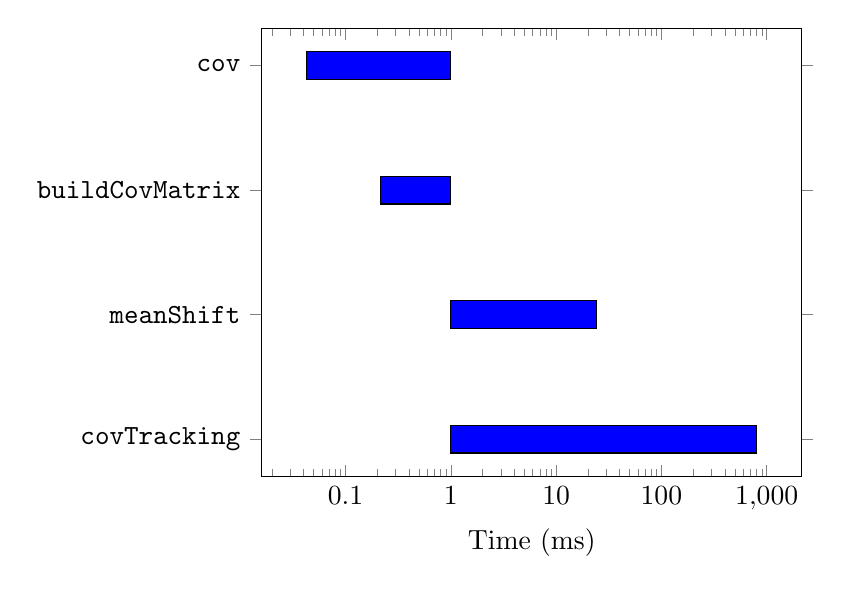
\begin{tikzpicture}
\begin{axis}[
    xbar,
    symbolic y coords={\texttt{covTracking},\texttt{meanShift},\texttt{buildCovMatrix},\texttt{cov}},
    xmode=log,
    log ticks with fixed point,
    xlabel={Time (ms)},
    ]
    \addplot[fill=blue] coordinates {
        (800.569,\texttt{covTracking})
        (24.276,\texttt{meanShift})
        (0.214,\texttt{buildCovMatrix})
        (0.043,\texttt{cov})
    };
\end{axis}
\end{tikzpicture}
\caption{Performance of our components. Our multi-scale covariance tracking takes an order of magnitude longer than mean-shift tracking.}\label{fig:perf}
\end{figure}

Figure~\ref{fig:perf} shows our algorithm's performance.\texttt{buildCovMatrix} is a subroutine inside of \texttt{covTracking} that constructs the covariance variance for each sliding window patch. \texttt{cov} is a subroutine inside of \texttt{buildCovMatrix} simply computes the covariance matrix $\Sigma$. It should be noted that \texttt{buildCovMatrix} and \texttt{cov} are called thousands of times, on average, since we must construct the covariance matrix for each location in the search area. This is where the bulk of the time is spent. The multi-scale covariance tracking clearly takes the longest amount of time. Mean-shift tracking, even with a large number of iterations, takes an order of magnitude less time than covariance tracking. Our algorithm's performance scales linearly if we reduce the number of scaling factors.

\begin{table}[t]
\centering
\begin{tabular}{lccccccc}
\toprule
\textbf{Radius} & \textbf{tp} & \textbf{fp} & \textbf{tn} & \textbf{fn} & \textbf{Precision} & \textbf{Recall} & \textbf{Accuracy} \\
\midrule
3 & 8 & 7 & 15 & 10 & 0.5333 & 0.4444 & 0.5750\\
5 & 10 & 7 & 12 & 11 & 0.5882 & 0.4762 & 0.5500\\
7 & 5 & 5 & 12 & 18 & 0.5000 & 0.2174 & 0.4250\\
20 & 5 & 5 & 10 & 20 & 0.5000 & 0.2000 & 0.2500\\
\bottomrule
\end{tabular}
\caption{Confusion matrices for varying neighborhood sizes. Smaller neighborhood size results in better quality.}\label{fig:accuracy}
\end{table}

Table~\ref{fig:accuracy} shows our algorithm's precision, recall, accuracy, as well as the confusion matrices, as a function of the neighborhood radius of the mean-shift tracking algorithm. Since we had no ground-truth data, we randomly sampled $40$ frames and had a human judge if the bounding box was on the target, i.e., the van. In our specific case, precision means, from the detected events, i.e., the ``positives'', the target is correctly inside of the bounding box, and, recall means our algorithm correctly detected the target whenever it was actually there.

We see that using a smaller mean-shift neighborhood radius produces better precision and recall in the other cameras. However, in the primary camera, mean-shift tracking suffers as a result. The smaller neighborhood radius is also more appropriate for the dimensions of the camera feed.

\subsection{Lessons Learned}
\vspace{5pt}
\noindent\textbf{Vectorize code.} Vectorized code tends to run faster than non-vectorized code due to parallelism and efficient algorithms for large matrix multiplication. We learned that a good approach is to start without vectorized code and remove loops by condensing data structures into matrices or tensors. Tensor arithmetic is also noticeably faster than non-vectorized code.

\vspace{5pt}
\noindent\textbf{Use camera calibration files.} Many datasets we found with provided their own camera calibration numbers. Working with these matrices is not entirely straightforward at times. Furthermore, point matching for computing the homography can be quite time-consuming. We need to manually select good corresponding points to use for the homography if feature detectors do not select good homography points. Automated approaches exist, but the perspective difference between the two camera is large enough that many of these don't work.

\vspace{5pt}
\noindent\textbf{Account for drift.} Mean-shift tracking point tends to drift in the primary camera. This can drastically affect the projection of the points into another camera frame. A small change in position in the primary camera might lead to a large movement in another camera. This drastically affects the quality of the result: if we use a constant size search area, then a large jump may cause the target to be outside of the search region. One solution is varying the search area size as a function of the Euclidean distance between the last two positions of mean-shift tracking, i.e., use a larger search area if the tracked point jumped far and vice-versa.

\section{Future Work}
\label{sec:future}
\vspace{5pt}
\noindent\textbf{Narrow search space with an object detector.} Instead of creating the search space from the projected points, we can reduce our search space even further by running a object detector, such as Faster R-CNN~\cite{ren2015faster}, YOLO~\cite{redmon2016you}, or Single-Shot Detector~\cite{liu2016ssd}, on each non-primary camera. These models draw bounding boxes on each object in a frame, depending on the frame rate. Then we can check the box of the $k$-closest objects to the transformed points.

\vspace{5pt}
\noindent\textbf{Construct a visual hull.} Knowing the locations of cameras in 3D space allows us to use an algorithm, such as VisualHull~\cite{laurentini1994visual}, to construct a complete 3D wireframe of the target. This provides additional information, such as target height, that may be used to help narrow searching or constructing a description of the target.

\vspace{5pt}
\noindent\textbf{Dynamic camera switching.} One useful feature for an application of multi-camera tracking is dynamically switching between cameras that have lost and captured the target. For example, if a target is no longer visible in one camera, remove the camera feed from the application dashboard. If it is picked up in another camera, add the camera feed to the dashboard. This allows the user to keep track of all cameras on the target without having to search through many different camera feeds.

\bibliographystyle{abbrv}
\bibliography{biblio}

\end{document}
